\section{5-state Sporadic Machines}\label{sec:sporadic}



\begin{figure}[h!]
    \centering

    % First row: 3 images
    \begin{minipage}{\textwidth}
        \centering
        \begin{subfigure}{0.3\textwidth}
            \centering
            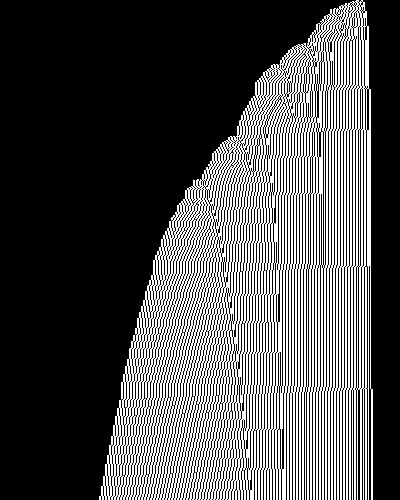
\includegraphics[width=\linewidth]{figures/sporadic-machines/sk1.png}
            \caption*{\href{https://bbchallenge.org/1RB1RD_1LC0RC_1RA1LD_0RE0LB_---1RC}{Skelet \#1}}
        \end{subfigure}
        \hfill
        \begin{subfigure}{0.3\textwidth}
            \centering
            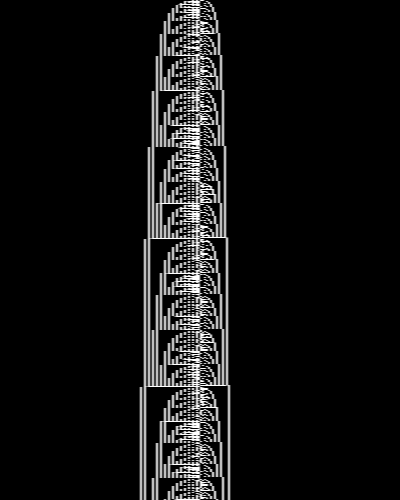
\includegraphics[width=\linewidth]{figures/sporadic-machines/sk10.png}
            \caption*{\href{https://bbchallenge.org/1RB0RA_0LC1RA_1RE1LD_1LC0LD_---0RB}{Skelet \#10}}
        \end{subfigure}
        \hfill
        \begin{subfigure}{0.3\textwidth}
            \centering
            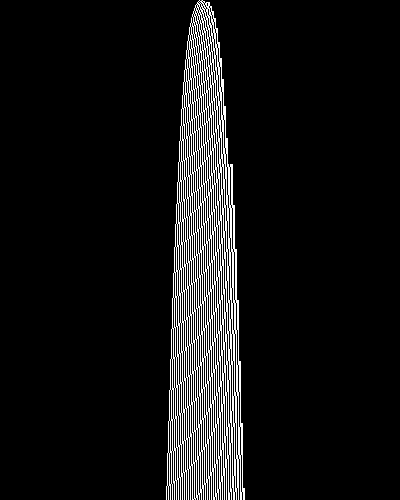
\includegraphics[width=\linewidth]{figures/sporadic-machines/sk17.png}
            \caption*{\href{https://bbchallenge.org/1RB---_0LC1RE_0LD1LC_1RA1LB_0RB0RA}{Skelet \#17}}
        \end{subfigure}
    \end{minipage}

    \vspace{1.5em}

    % Second row: Shift Overflow Counters
    \begin{tikzpicture}
        \node[draw=magenta, thick, rounded corners, inner sep=8pt] (box1) {
            \begin{minipage}{0.95\textwidth}
                \centering
                \textbf{\textcolor{magenta}{Shift Overflow Counters}}\\[0.8em]
                \begin{subfigure}{0.17\textwidth}
                    \centering
                    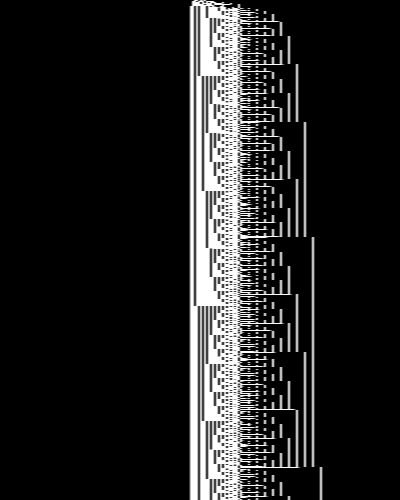
\includegraphics[width=\linewidth]{figures/sporadic-machines/soc_sk15.png}
                    \caption*{\href{https://bbchallenge.org/1RB---_1RC1LB_1LD1RE_1LB0LD_1RA0RC}{Skelet \#15}}
                \end{subfigure}
                \hfill
                \begin{subfigure}{0.17\textwidth}
                    \centering
                    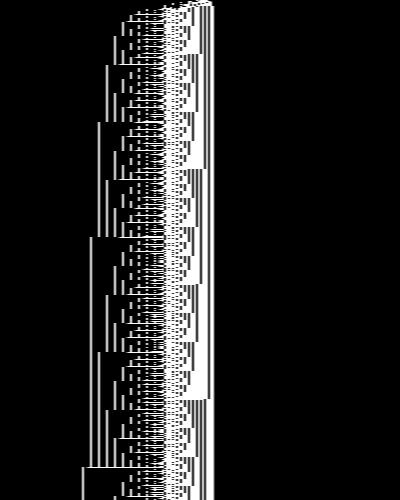
\includegraphics[width=\linewidth]{figures/sporadic-machines/soc_sk26.png}
                    \caption*{\href{https://bbchallenge.org/1RB1LD_1RC0RB_1LA1RC_1LE0LA_1LC---}{Skelet \#26}}
                \end{subfigure}
                \hfill
                \begin{subfigure}{0.17\textwidth}
                    \centering
                    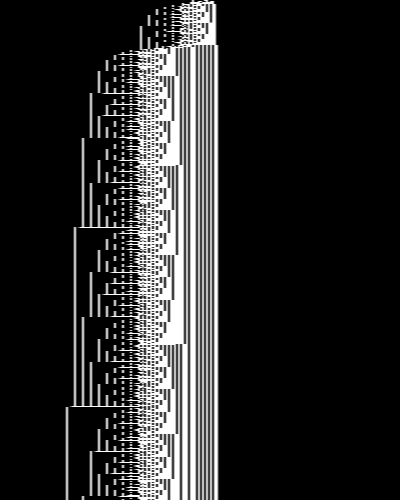
\includegraphics[width=\linewidth]{figures/sporadic-machines/soc_sk33.png}
                    \caption*{\href{https://bbchallenge.org/1RB1LC_0RC0RB_1LD0LA_1LE---_1LA1RE}{Skelet \#33}}
                \end{subfigure}
                \hfill
                \begin{subfigure}{0.17\textwidth}
                    \centering
                    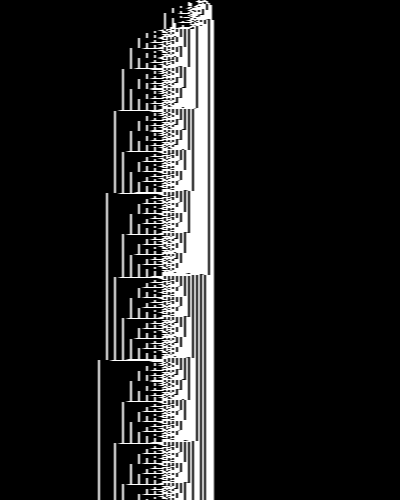
\includegraphics[width=\linewidth]{figures/sporadic-machines/soc_sk34.png}
                    \caption*{\href{https://bbchallenge.org/1RB1LC_0RC0RB_1LD0LA_1LE---_1LA1RA}{Skelet \#34}}
                \end{subfigure}
                \hfill
                \begin{subfigure}{0.17\textwidth}
                    \centering
                    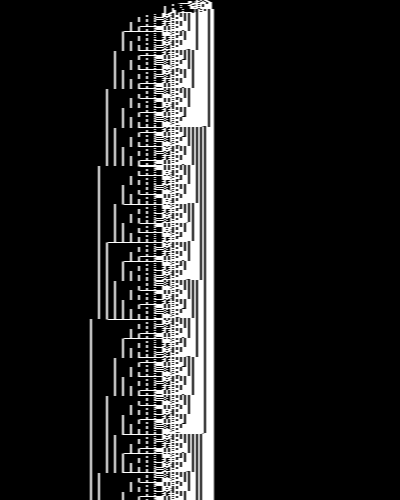
\includegraphics[width=\linewidth]{figures/sporadic-machines/soc_sk35.png}
                    \caption*{\href{https://bbchallenge.org/1RB1LC_0RC0RB_1LD0LA_1LE---_1LA0LA}{Skelet \#35}}
                \end{subfigure}
            \end{minipage}
        };
    \end{tikzpicture}

    \vspace{1.5em}

    % Third row: Finned Machines
    \begin{tikzpicture}
        \node[draw=magenta, thick, rounded corners, inner sep=8pt] (box2) {
            \begin{minipage}{0.95\textwidth}
                \centering
                \textbf{\textcolor{magenta}{Finned Machines}}\\[0.8em]
                \begin{subfigure}{0.17\textwidth}
                    \centering
                    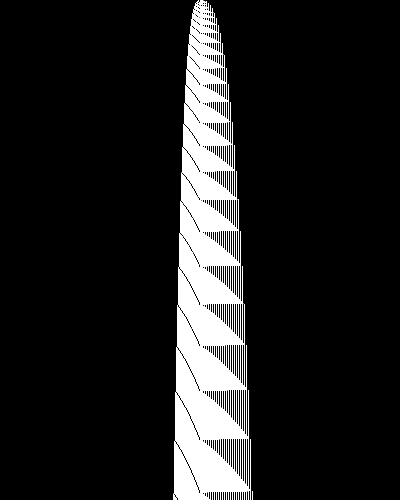
\includegraphics[width=\linewidth]{figures/sporadic-machines/finned_1.png}
                    \caption*{\href{https://bbchallenge.org/1RB0LE_1RC1RB_1RD1LC_0LE0RB_---1LA}{Finned \#1}}
                \end{subfigure}
                \hfill
                \begin{subfigure}{0.17\textwidth}
                    \centering
                    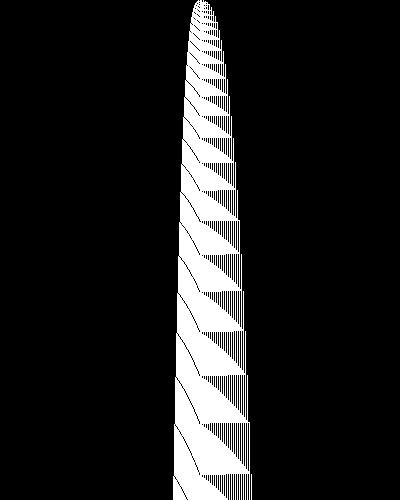
\includegraphics[width=\linewidth]{figures/sporadic-machines/finned_2.png}
                    \caption*{\href{https://bbchallenge.org/1RB1RA_1RC1LB_0LD0RA_1RA1LE_---0LD}{Finned \#2}}
                \end{subfigure}
                \hfill
                \begin{subfigure}{0.17\textwidth}
                    \centering
                    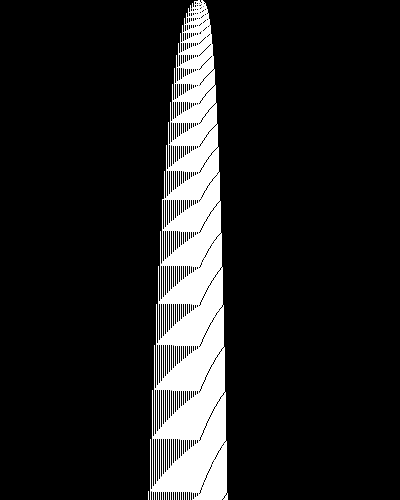
\includegraphics[width=\linewidth]{figures/sporadic-machines/finned_3.png}
                    \caption*{\href{https://bbchallenge.org/1RB1RE_1LC1RB_0RA0LD_1LB1LD_---0RA}{Finned \#3}}
                \end{subfigure}
                \hfill
                \begin{subfigure}{0.17\textwidth}
                    \centering
                    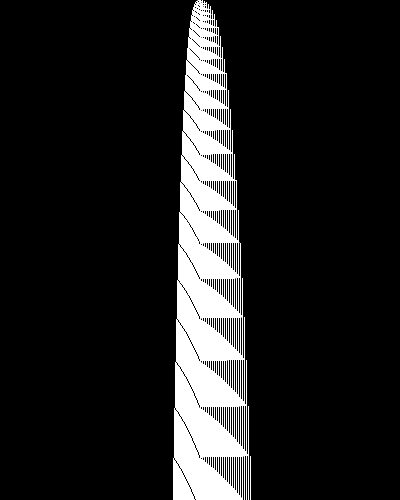
\includegraphics[width=\linewidth]{figures/sporadic-machines/finned_4.png}
                    \caption*{\href{https://bbchallenge.org/1RB1LA_0LC0RE_---1LD_1RA0LC_1RA1RE}{Finned \#4}}
                \end{subfigure}
                \hfill
                \begin{subfigure}{0.17\textwidth}
                    \centering
                    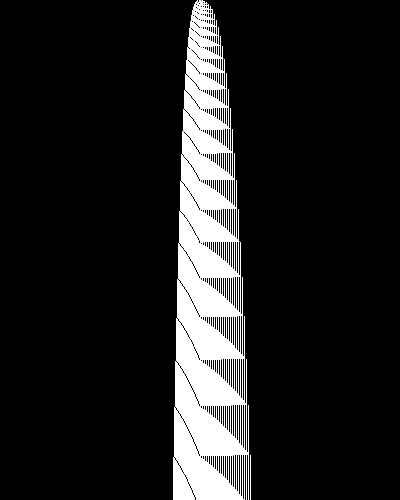
\includegraphics[width=\linewidth]{figures/sporadic-machines/finned_5.png}
                    \caption*{\href{https://bbchallenge.org/1RB1LA_0LC0RE_---1LD_1LA0LC_1RA1RE}{Finned \#5}}
                \end{subfigure}
            \end{minipage}
        };
    \end{tikzpicture}

    \caption{{\small Family picture of the 5-state Sporadic Machines (20,000-step space-time diagrams) which required individual \Coq nonhalting proofs; machine names in the Figure are clickable URLs giving the TNF-normalised transition table of each machine (see Section~\ref{sec:enum}). All Sporadic Machines were also identified by Skelet \cite{Skelet_bbfind}, either as unprovable using his \texttt{bbfind} program, or, for what we call ``Finned Machines'' marked as ``easily provable by hand'' \cite{Skelet_bbfind_list}. For better visibility, diagrams of counters (Skelet \#10 and Shift Overflow Counters) have been represented using a tape of length 200 instead of 400, giving a \textit{zoomed-in} effect.}}
    \label{fig:sporadic}
\end{figure}

Sporadic Machines are 13 nonhalting 5-state Turing machines that were not captured by deciders (Section~\ref{sec:deciders}) and required individual \Coq proofs of nonhalting; their space-time diagrams are given in Figure~\ref{fig:sporadic}. Twelve of these machines, \ie all but ``Skelet \#17'' (see below), were proved nonhalting in \texttt{busycoq} \cite{busycoq}, and then integrated\footnote{For convenience, the relevant parts of \texttt{busycoq} have been added to the root of \CoqBB, at \url{https://github.com/ccz181078/Coq-BB5/tree/main/BusyCoq}. \CoqBB translates \texttt{busycoq} proofs using \href{https://github.com/ccz181078/Coq-BB5/blob/main/CoqBB5/BB5/BusyCoq_Translation.v}{\texttt{BusyCoq\_Translation.v}}.} into \CoqBB. Machine ``Skelet \#17'' was the last 5-state machine to be formally proven nonhalting in Coq, as part of \CoqBB, achieving the proof of $S(5) = \BBtheFifth$ -- a different proof also had been released as a standalone paper, \cite{xu2024skelet17fifthbusy}.

Interestingly all Sporadic Machines had been identified by Georgi Georgiev (also known as ``Skelet'', see Section~\ref{sec:intro:mainresults}) in 2003: either as part of his 43 unsolved machines\footnote{Apart from \cite{Skelet_bbfind_list}, these 43 machines are also listed here: \url{https://bbchallenge.org/skelet}.} which are named after him, \eg ``Skelet \#1'' (see Figure~\ref{fig:sporadic}), either, in the case of what we call ``Finned Machines'', marked by him as ``easily provable by hand'' \cite{Skelet_bbfind_list}. In 2010, an effort to mathematically prove Skelet's machines nonhalting was initiated by Briggs which influenced \texttt{busycoq}'s proof of machine ``Skelet \#10'' \cite{DanBriggs}. Sporadic Machines can be arranged in three buckets:
\begin{itemize}
    \item \textbf{Finned Machines.} These are five akin machines that were solved by handcrafting nonhalting certificates similar in flavor to WFAR certificates (Section~\ref{sec:WFAR}). The certificates were crafted by Blanchard, translated in \Coq by mei, see \texttt{busycoq} files \texttt{Finned\{1-5\}.v}. An argument of irregularity (Section~\ref{sec:deciders-overview}) was given for machine ``Finned \#3'' \cite{irregularFinned3}. A later-developed irregular extension of RepWL (Section~\ref{sec:RepWL}) has been reported to solve these machines\footnote{\url{https://discuss.bbchallenge.org/t/bb5s-finned-machines-summary/234}}.
    \item \textbf{Shift Overflow Counters.} This family concerns Skelet's machines 15, 26, 33, 34 and 35; Figure~\ref{fig:sporadic}. These machines are similar: dividing the tape in two, they implement two independent binary counters, one on each side, and they undergo relatively complex behaviors when either counter overflows. They have been described in details by Ligocki, who first analysed them \cite{ShawnSOC}. They were then proved in \Coq by Yuen and mei as part of \texttt{busycoq} \cite{busycoq}.
    \item \textbf{Skelet \#1, Skelet \#10, and, Skelet \#17.} These three machines have really unique behaviors which we detail below.
\end{itemize}

\paragraph{Skelet \#1.}

\paragraph{Skelet \#10.}

\paragraph{Skelet \#17.}